\section{INFORMACIÓN CONTEXTUAL EN LOS SISTEMAS DE RECOMENDACIÓN}

La forma en que se ha abordado el problema principal de los sistemas de recomendación ha evolucionado a lo largo del tiempo, sin embargo, la mayoría de investigaciones se enfocan en la interacción \textit{item - usuario} o \textit{usuario - item} y no se suele tomar en cuenta ningún tipo de contexto adicional que podría alterar la calidad de las recomendaciones.

Sin embargo, con la evolución de los Sistemas de Recomendación, ha surgido la necesidad de categorizar a los sistemas que son \textbf{sensibles al contexto} para encontrar métodos y enfoques que logren brindar al sistema la información necesaria para entender las necesidades y preferencias del usuario. Estos sistemas de recomendación sensibles al contexto se definen formalmente como \textit{Context-Aware recommender systems (CARS)}. 

\begin{definition}

En los sistemas de recomendación, el \textbf{Contexto} se puede definir como cualquier información que puede ser usada para caracterizar la situación de una entidad, donde una entidad puede representar a una persona, un lugar o un objeto computacional. Esta información adicional puede ayudar al sistema a ser más preciso. \mbox{\parencite{mateos2024systematic}}.

\end{definition}

Los \textit{CARS} son aquellos sistemas que buscan entender las preferencias del usuario incorporando información contextual en el proceso de recomendación. Esto implica que una calificación dada por el usuario ahora es afectada también por el contexto en el que se realizó. Por lo tanto, según \parencite{10.5555/1941884}, una \textit{calificación} ahora se puede definir de la siguiente manera:

\begin{equation}
    Usuario \times Item \times Contexto \rightarrow Calificacion
    \addequation{Cálculo de Calificación mediante un Contexto}
\end{equation}

Es importante mencionar que el Contexto puede definir diferentes aspectos del contexto del sistema ya sea tiempo, localización, compañía, propósito, y muchos más. 

\newpage

\subsection{PREFILTRADO CONTEXTUAL}

En el \textit{Prefiltrado Contextual} el contexto específico determinará qué información es la más relevante respecto a las preferencias del usuario, obteniendo un subconjunto de elementos que servirá como base para obtener recomendaciones mediante los algorítmos de recomendación clásicos.
El prefiltrado de items mediante contexto aumenta la diversidad de recomendaciones gracias a la división de datos en diferentes escenarios contextuales, sin embargo, tratar de recrear un contexto específico puede llevar a un problema de \textbf{escasez de datos}, obteniendo una recomendación altamente limitada \parencite{mateos2024systematic}.

En general, cuando se busca desarrollar un sistema de recomendación, usar un prefiltrado contextual puede resultar en desventajas importantes que afectan al desempeño del sistema, principalmente si se busca un enfoque generalizable a distintos dominios. A pesar de sus limitaciones en escenarios generales, el prefiltrado sigue siendo útil cuando se diseña en campos específicos.

\subsection{HEURÍSTICAS DE PREFILTRADO}

Para obtener un subconjunto relevante de items se suelen usar diversas técnicas de prefiltrado, una de ellas es el uso de \textbf{Heurísticas}.

\begin{definition}
    Las \textbf{Heurísticas} son criterios, métodos o principios para decidir entre diversas ramas de acción a aquella que prometa ser la más efectiva para lograr cierto propósito. Una heurística podría ser un atajo usado para guiar cierta acción \parencite{Pearl1984}.
\end{definition}

El objetivo de una Heurística no es garantizar la mejor solución a un problema, sino proponer una solución \textbf{suficientemente buena} en un tiempo razonable. En el caso de los sistemas de recomendación sensibles al contexto, las heurísticas permiten seleccionar de manera rápida un subconjunto de ítems relevantes para un usuario bajo un contexto particular, obteniendo una muestra significativa sobre el cual podrían operar los algorítmos de recomendación tradicionales.

\begin{definition}
    Los \textbf{Algorítmos Heurísticos} son una clase de algorítmos matemáticos que utilizan diversas técnicas heurísticas para la resolución de problemas complejos \parencite{proy2024algoritmos}.
\end{definition}

Las técnicas heurísticas más importantes para los algorítmos propuestos en el presente proyecto son las \textit{heurísticas voraces} y las \textit{heurísticas tabú}.

Antes de explicar de manera detallada estas heurísticas, es importante comprender el concepto de \textbf{espacio de estados} y \textbf{Funciones Heurísticas}. 

\begin{definition}
    El \textbf{espacio de estados} es el conjunto de todas las posibles configuraciones o situaciones que un sistema o problema puede alcanzar. Cada \textbf{estado} representa una situación particular del sistema, y una \textbf{transición} representa una acción o movimiento permitido con un costo asociado \parencite{heusner2017understanding}.
\end{definition}

En ciertos algorítmos el \textit{espacio de estados} es un conjunto predefinido que representa el espacio total con el que se trabajará, sin embargo, igualmente existen \textbf{modelos generativos de espacio de estados} que generan estados bajo demanda en lugar de tenerlos definidos desde el inicio. Los \textbf{modelos generativos} brindan la posibilidad de explorar \textbf{espacios grandes} sin necesidad de procesar toda la información. Estos algoritmos se apoyan en la estimación de costos o distancias entre estados para decidir cuál estado expandir en cada paso.

\begin{definition}
    Las \textbf{Funciones Heurísticas} son funciones que estiman el \textbf{costo} o \textbf{distancia} desde el estado inicial hasta el estado final \parencite{heusner2017understanding}.
\end{definition}

Las funciones heurísticas nos permiten estimar el costo o distancia entre estados mediante cálculos o procedimientos algorítmicos, sin embargo, en muchas ocasiones son llamadas \textit{cajas negras} ya que, en ciertas situaciones, no importa cómo calcula la heurística, solo importa la información que retorna.

\subsubsection{HEURÍSTICAS VORACES (GREEDY)}
Los \textit{Algorítmos Voraces} representan una estrategia para generar soluciones \textit{suboptimas} mediante ramas de decisiones irrevocables. Cada una de estas decisiones representa la mejor opción en el momento en que se toman \parencite{khuller2018greedy}.

En el ámbito de la algorítmia, los algorítmos voraces son usados para encontrar respuestas \textbf{máximas} o \textbf{mínimas} a un problema. Sin embargo, en sistemas complejos, también suelen ser usados para obtener soluciones \textbf{aproximadas} encontrando respuestas que podrían ser \textit{subóptimas} pero cumpliendo con un mínimo de rendimiento. 

A continuación se describen algunos algorítmos clásicos que utilizan heurísticas voraces para la exploración del espacio de estados.

\newpage

\textbf{ALGORÍTMO VORÁZ DE BÚSQUEDA POR NIVELES}

El \textit{Algorítmo Voráz de Búsqueda a Profundiad} o \textit{(GBFS)} es un algorítmo de búsqueda informada y voráz que intenta alcanzar la meta priorizando los estados que parecen más cercanos según la heurística, aunque no garantiza el costo mínimo total. Recibe como entrada un \textit{espacio de estados} estático o generativo y devuelve un plan que alcanza la meta sin embargo, existen casos \textit{insolubles} que indican que no se puede llegar a la meta.

Según \parencite{heusner2017understanding} la \textit{GBFS} se basa en la suposición de que los estados con menor \textbf{valor heurístico} (costo) forman parte del camino más barato hacia la meta, por esta razón se considera un \textit{algoritmo voráz}. Este algoritmo no necesita conocer todo el espacio de estados para funcionar debido a que únicamente opera en los estados que ya han sido generados. En cada paso el estado actual se expande al que tiene el \textit{menor valor heurístico} entre todos los estados que han sido generados que no han sido visitados previamente, esto se repite hasta generar el estado destino. 

Este criterio \textit{voráz} es la razón por la que este algoritmo no genera las soluciones más cortas debido a que en la mayoría de casos una decisión local no es suficiente para predecir el mejor resultado global, inclusive, no hay garantías de que el resultado tenga un mínimo de calidad. Debido a la inexactitud de la heurística, \textit{GBFS} puede quedarse atrapado en mesetas donde muchos estados tienen el mismo valor heurístico, o en mínimos locales donde la heurística guía hacia caminos no óptimos, lo que puede aumentar el tiempo de búsqueda o producir soluciones subóptimas.

\begin{figure}[h!]
    \centering
    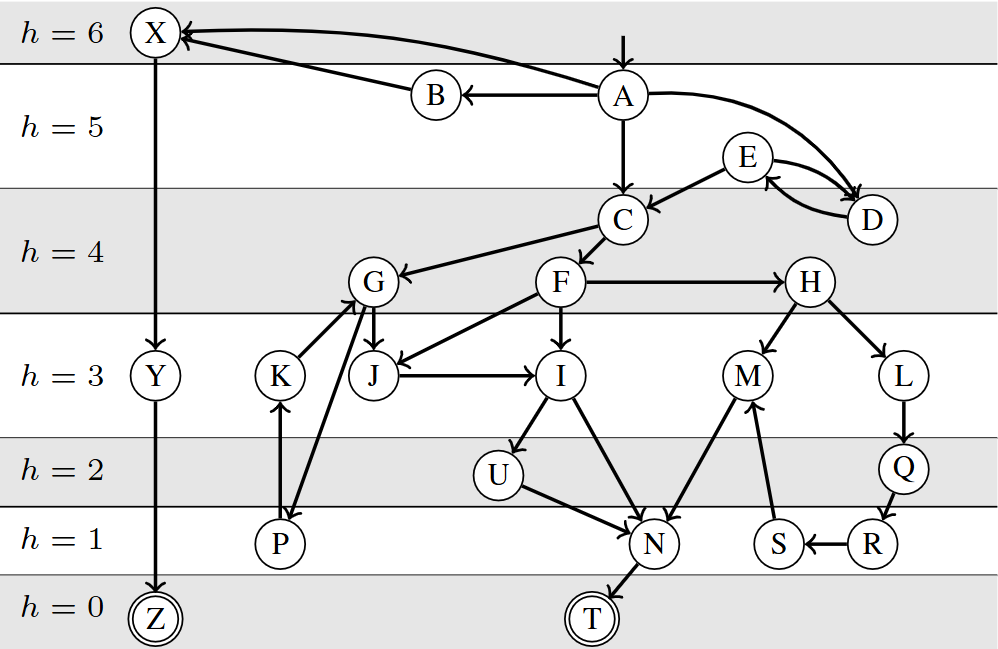
\includegraphics[width=0.7\linewidth]{EjemploDeGBFS.png}
    \caption{Ejemplo de GBFS \parencite{heusner2017understanding}.}
    \label{fig:EjemploGBFS}
\end{figure}

En la \Cref{fig:EjemploGBFS} se define el estado inical el nodo $A$ y el nodo objetivo $Z$. Cada nivel horizontal indica el cálculo $h$ de la distancia mediante la \textit{función heurística}. Además, se puede ver que existen diferentes caminos para llegar al nodo $Z$ y \textit{GBFS} podría retornar un camino menos óptimo como el más prometedor.

\textbf{ALGORITMO DE BÚSQUEDA A*}

El algoritmo \textit{A*} es un algoritmo que aprovecha una \textit{función heurística} para guiar su búsqueda hacia el nodo objetivo. Este algoritmo combina los mejores aspectos del \textit{Algoritmo Dijkstra}\footnote{\textbf{Algoritmo Dijkstra:} Algoritmo que encuentra el camino más corto a todos los nodos desde un único nodo orígen \parencite{javaid2013understanding}.} y \textit{GBFS} \parencite{KumarRAStar}. Esta combinación de algorítmos se puede definir de manera formal mediante la combinación de funciones $g(n)$ que representa el costo o distancia para alcanzar el nodo $n$ desde el nodo inicial, y $h(n)$ el costo de llegar desde un nodo $n$ hasta el nodo destino:

\begin{equation}
    f(n) = g(n) + h(n)
    \addequation{Definición de la función de A*}
\end{equation}

Así, $f(n)$ representa el costo estimado de la solución más barata que pase por el nodo $n$. Por lo tanto, si se busca encontrar la solución más barata, la estrategia es priorizar el nodo con el valor mínimo de $g(n) + h(n)$. Esta combinación es razonable y, junto a una buena \textit{función de heurística}, la \textit{búsqueda A*} garantiza soluciones óptimas \parencite{RusselArtificialIntelligence}. 

\begin{figure}[h!]
    \centering
    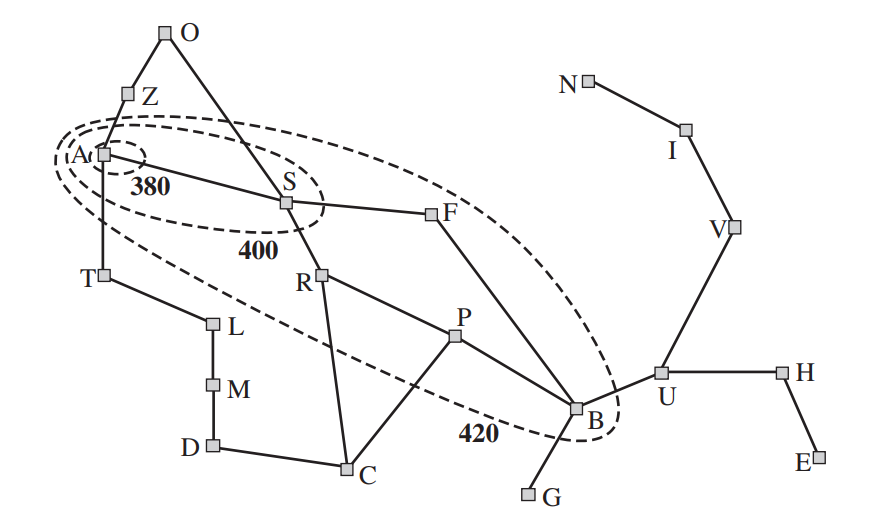
\includegraphics[width=0.8\linewidth]{EjemploASearch.png}
    \caption{Ejemplo del Algoritmo A* \parencite{RusselArtificialIntelligence}.}
    \label{fig:EjemploAStar}
\end{figure}

\newpage

En la \Cref{fig:EjemploAStar} se representa un problema clásico de inteligencia artíficial usado para explicar el algoritmo \textit{A*} llamado \textit{El Mapa de Rumanía}. Cada nodo representa una ciudad de Rumanía y las conexiones entre nodos representan las carreteras entre ciudades. El problema pide encontrar la ruta más corta desde \textit{Arad} hasta \textit{Bucarest}. En los contornos se muestran los valores $f(x)$ de los nodos que representan el camino más corto desde el inicio.

\subsubsection{HEURÍSTICAS TABÚ}




